\subsection{Experimentación sobre Kmeans}
\paragraph{}
Para los experimentos utilizamos las instancias de tipo A dadas por la cátedra. Los ejemplos de malos casos y problemas que puede llegar a tener kmeans fueron incluidos. Por ejemplo, los malos casos que acabamos de mencionar y sus diferentes tipos de entrada.
\paragraph{}
Para esta heurística y su experimentación tuvimos en cuenta principalmente dos cosas: el tamaño de la entrada y la forma en la que entran los datos o más directamente, como se recorren los puntos. Como vimos al analizar los casos, Kmeans depende de que centroids elige primero cuando la demanda es ajustada (recordemos la analogía de tetris que usamos). Por esto mismo, al experimentar sobre esta heurística decidimos tener en cuenta la forma en que se recorren los puntos (y en consecuencia, quienes tienen prioridad para asignarse a un cluster primero).
\paragraph{}
Una primera idea es ordenar los puntos por demanda, de manera decreciente. De esta forma, evitamos los casos en los que los camiones se van llenando de manera que quede bastante espacio en cada uno pero no el suficiente para albergar el producto de clientes de gran demanda. En casos en que esto no se tiene en cuenta, incluso podrían crearse nuevos clusters con centroid en esos clientes con alta demanda: lo cual puede significar en una mejora o no, dependiendo el caso. Por esto mismo, también decidimos experimentar con el caso contrario: en el que se de prioridad a los clientes con baja demanda, ordenando y recorriendo los puntos de manera creciente.
\paragraph{} 
Además de la experimentación mencionada, también chequeamos que la complejidad teórica que propusimos sea correcta o aproximada a la complejidad práctica del algoritmo.
\subsubsection{Sorting}

\begin{figure}[H]
	\centering
	\begin{minipage}{0.44\textwidth}
		\centering
		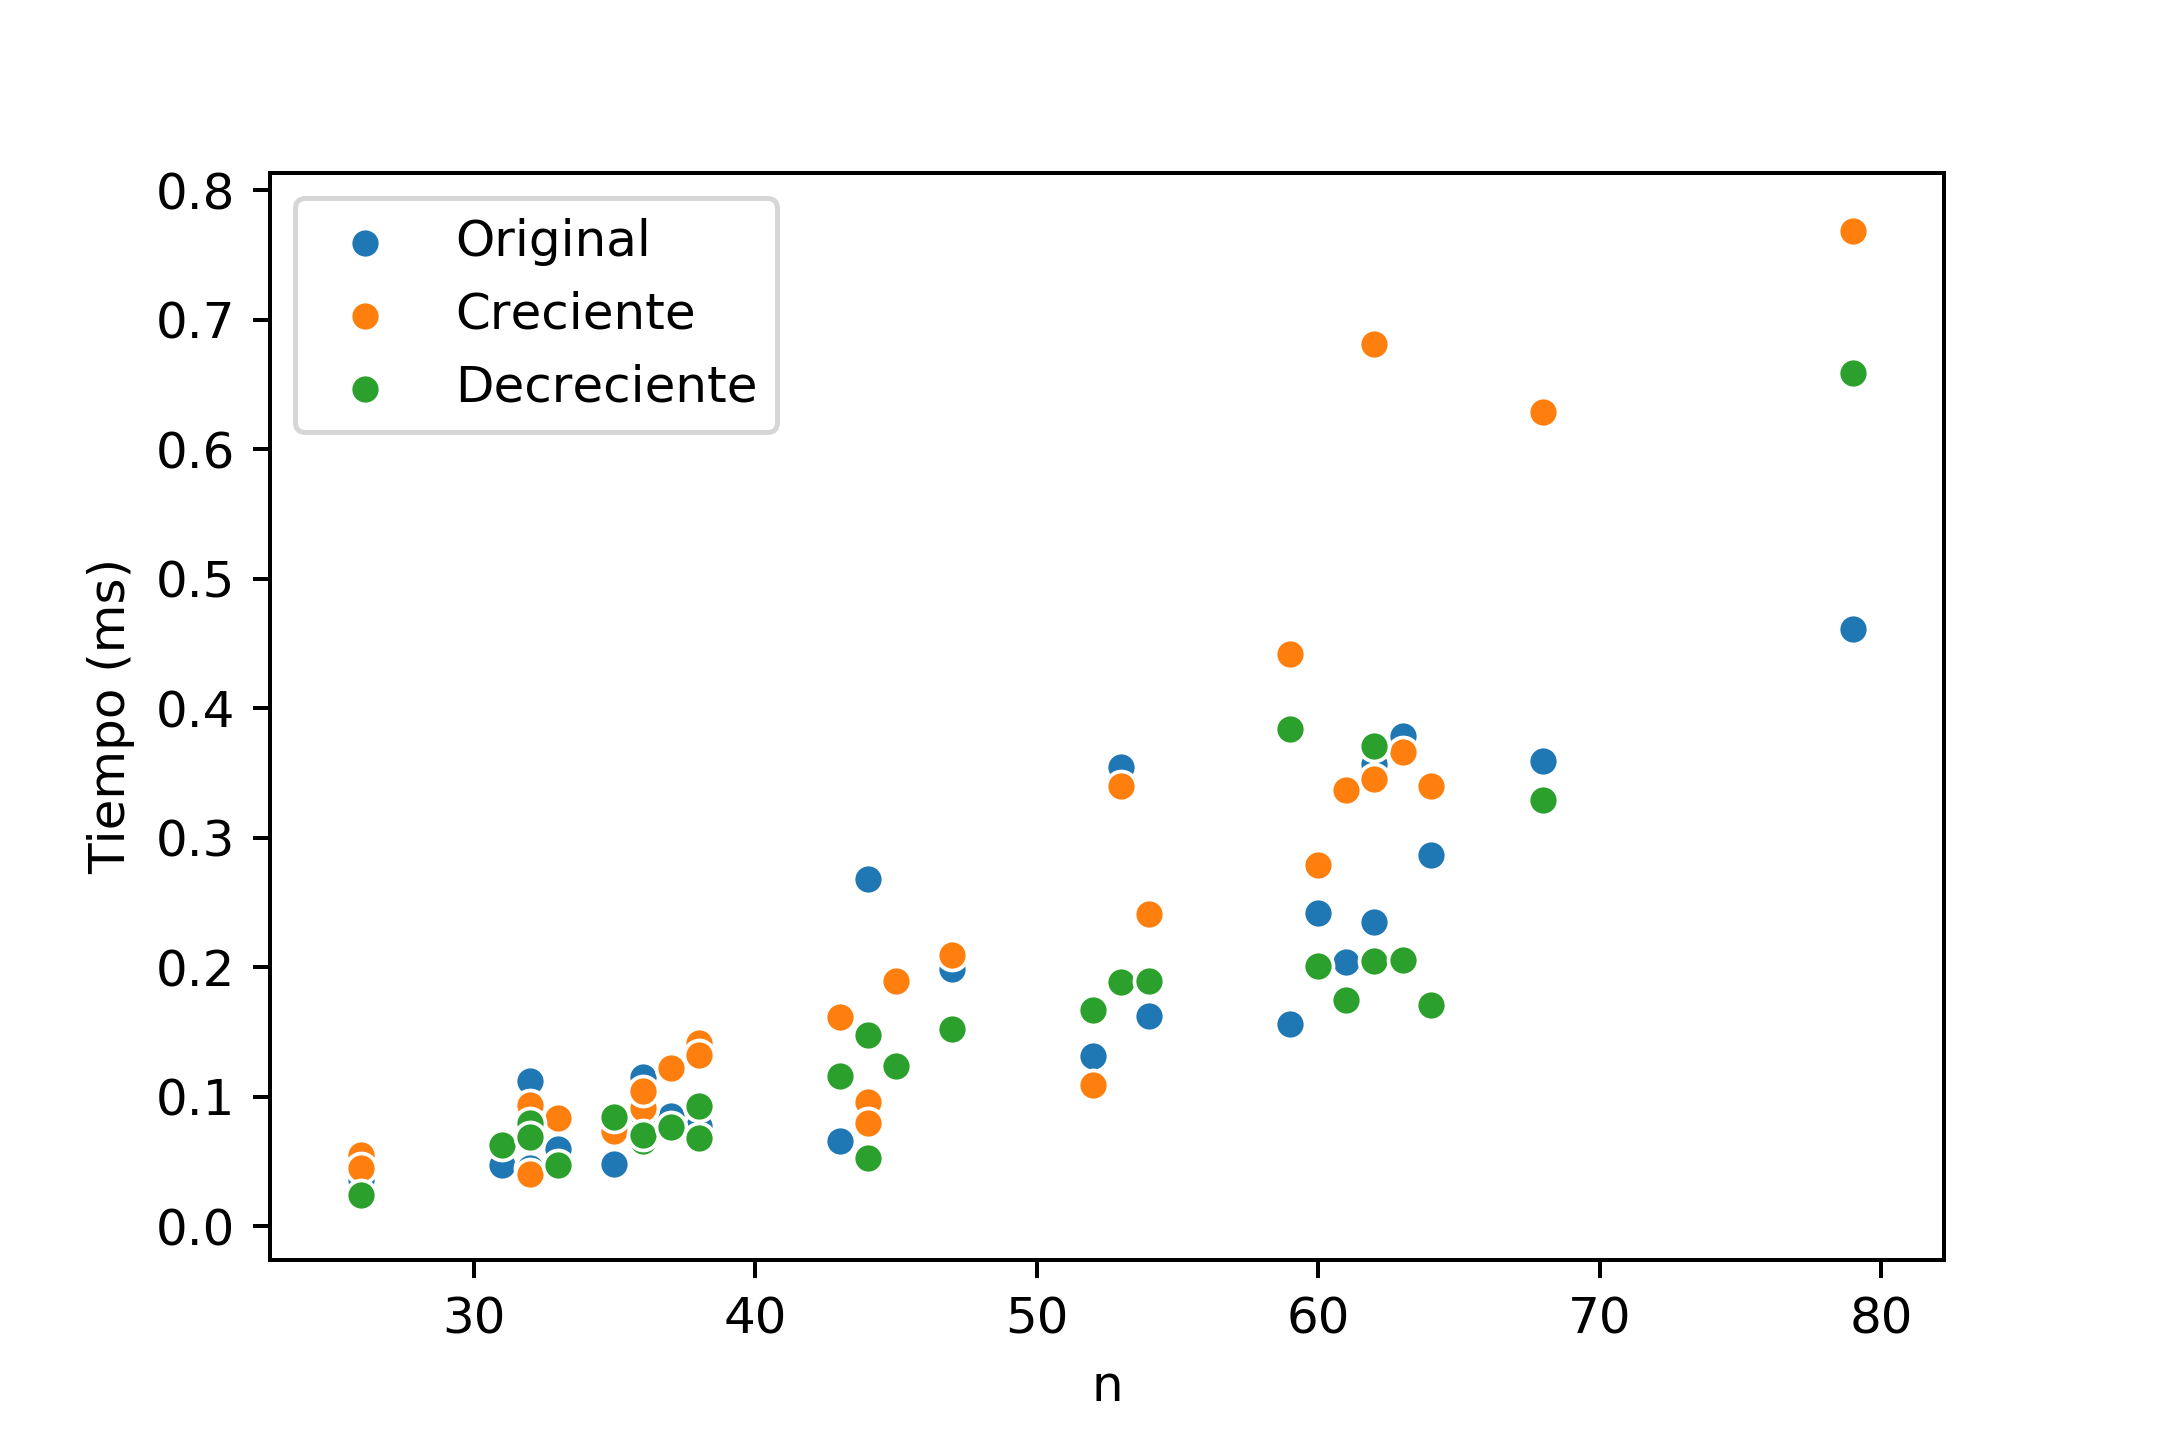
\includegraphics[width=1\textwidth]{images/kmeans/expsortingtiempo}
		\caption{\footnotesize Tiempo de acuerdo al tamaño de la entrada}
		\label{fig:kmeans-sort-tiempo}
	\end{minipage}%
	\hspace{0.03\textwidth}
	\begin{minipage}{0.44\textwidth}
		\centering
		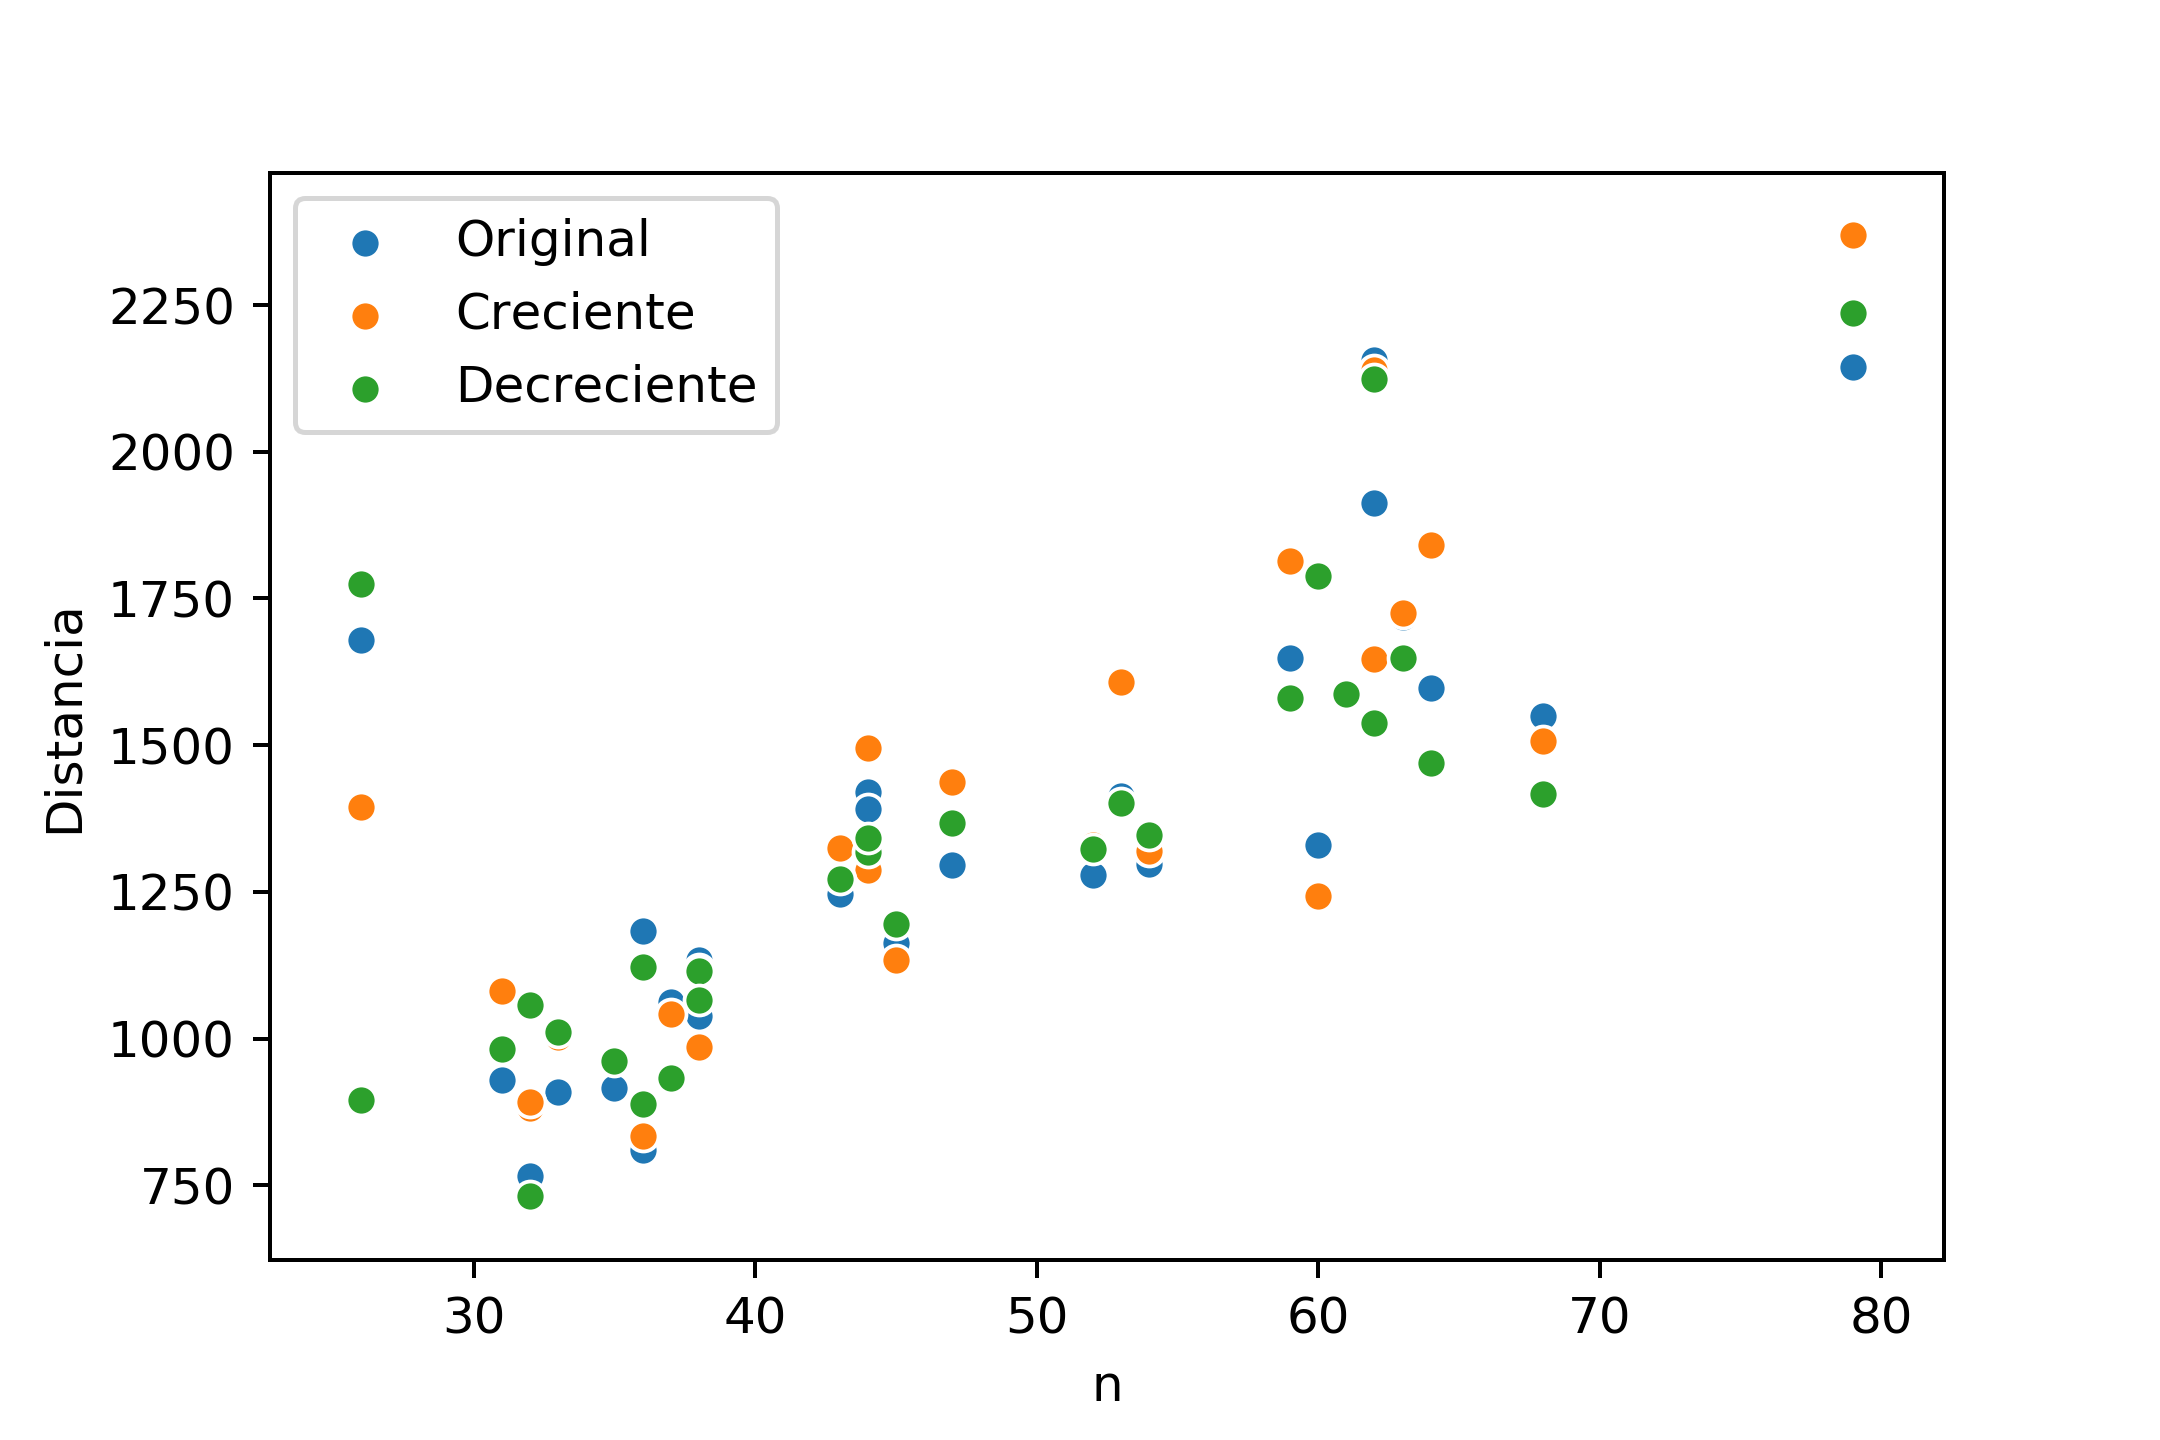
\includegraphics[width=1\textwidth]{images/kmeans/expsorting}
		\caption{\footnotesize Distancia de las soluciones obtenida de acuerdo al tamaño de la entrada}
		\label{fig:kmeans-sort-distancia}
	\end{minipage}%
\end{figure}
\paragraph{}
Finalmente, decidimos tener tres implementaciones de kmeans: donde recorra los puntos como vienen, donde ordene por demanda de forma decreciente y donde ordene de forma creciente. Como ordenar es $\mathcal{O}(n*log(n))$ hacer esto no altera la complejidad de la heurística. En la figura \ref{fig:kmeans-sort-tiempo} comparamos las performances de tiempo de los tres algoritmos. Se observa que al recorrer los puntos de forma decreciente el algoritmo toma menos tiempo: esto puede entenderse como que no se crean clusters nuevos ya que es más probable que al dar prioridad a los clientes con alta demanda, los de baja demanda puedan encajar en los espacios no tan grandes que quedan en los camiones al ir siendo ocupados. En general parece que efectivamente recorrerlos de forma creciente incrementa la cantidad de iteraciones y por eso toma más tiempo: más clusters, más cambios de pertenencia, etc.
\paragraph{}
Por otro lado, en \ref{fig:kmeans-sort-distancia} se compara que tan buenas son las soluciones entre sí. En esta experimentación, no se puede concluir que en cuanto a distancia mínima una implementación sea mejor o peor que otra: dependerá de como este formada la instancia que algoritmo conviene elegir. 
\subsubsection{Tiempos}

\begin{figure}[H]
	\centering
	\begin{minipage}{0.44\textwidth}
		\centering
		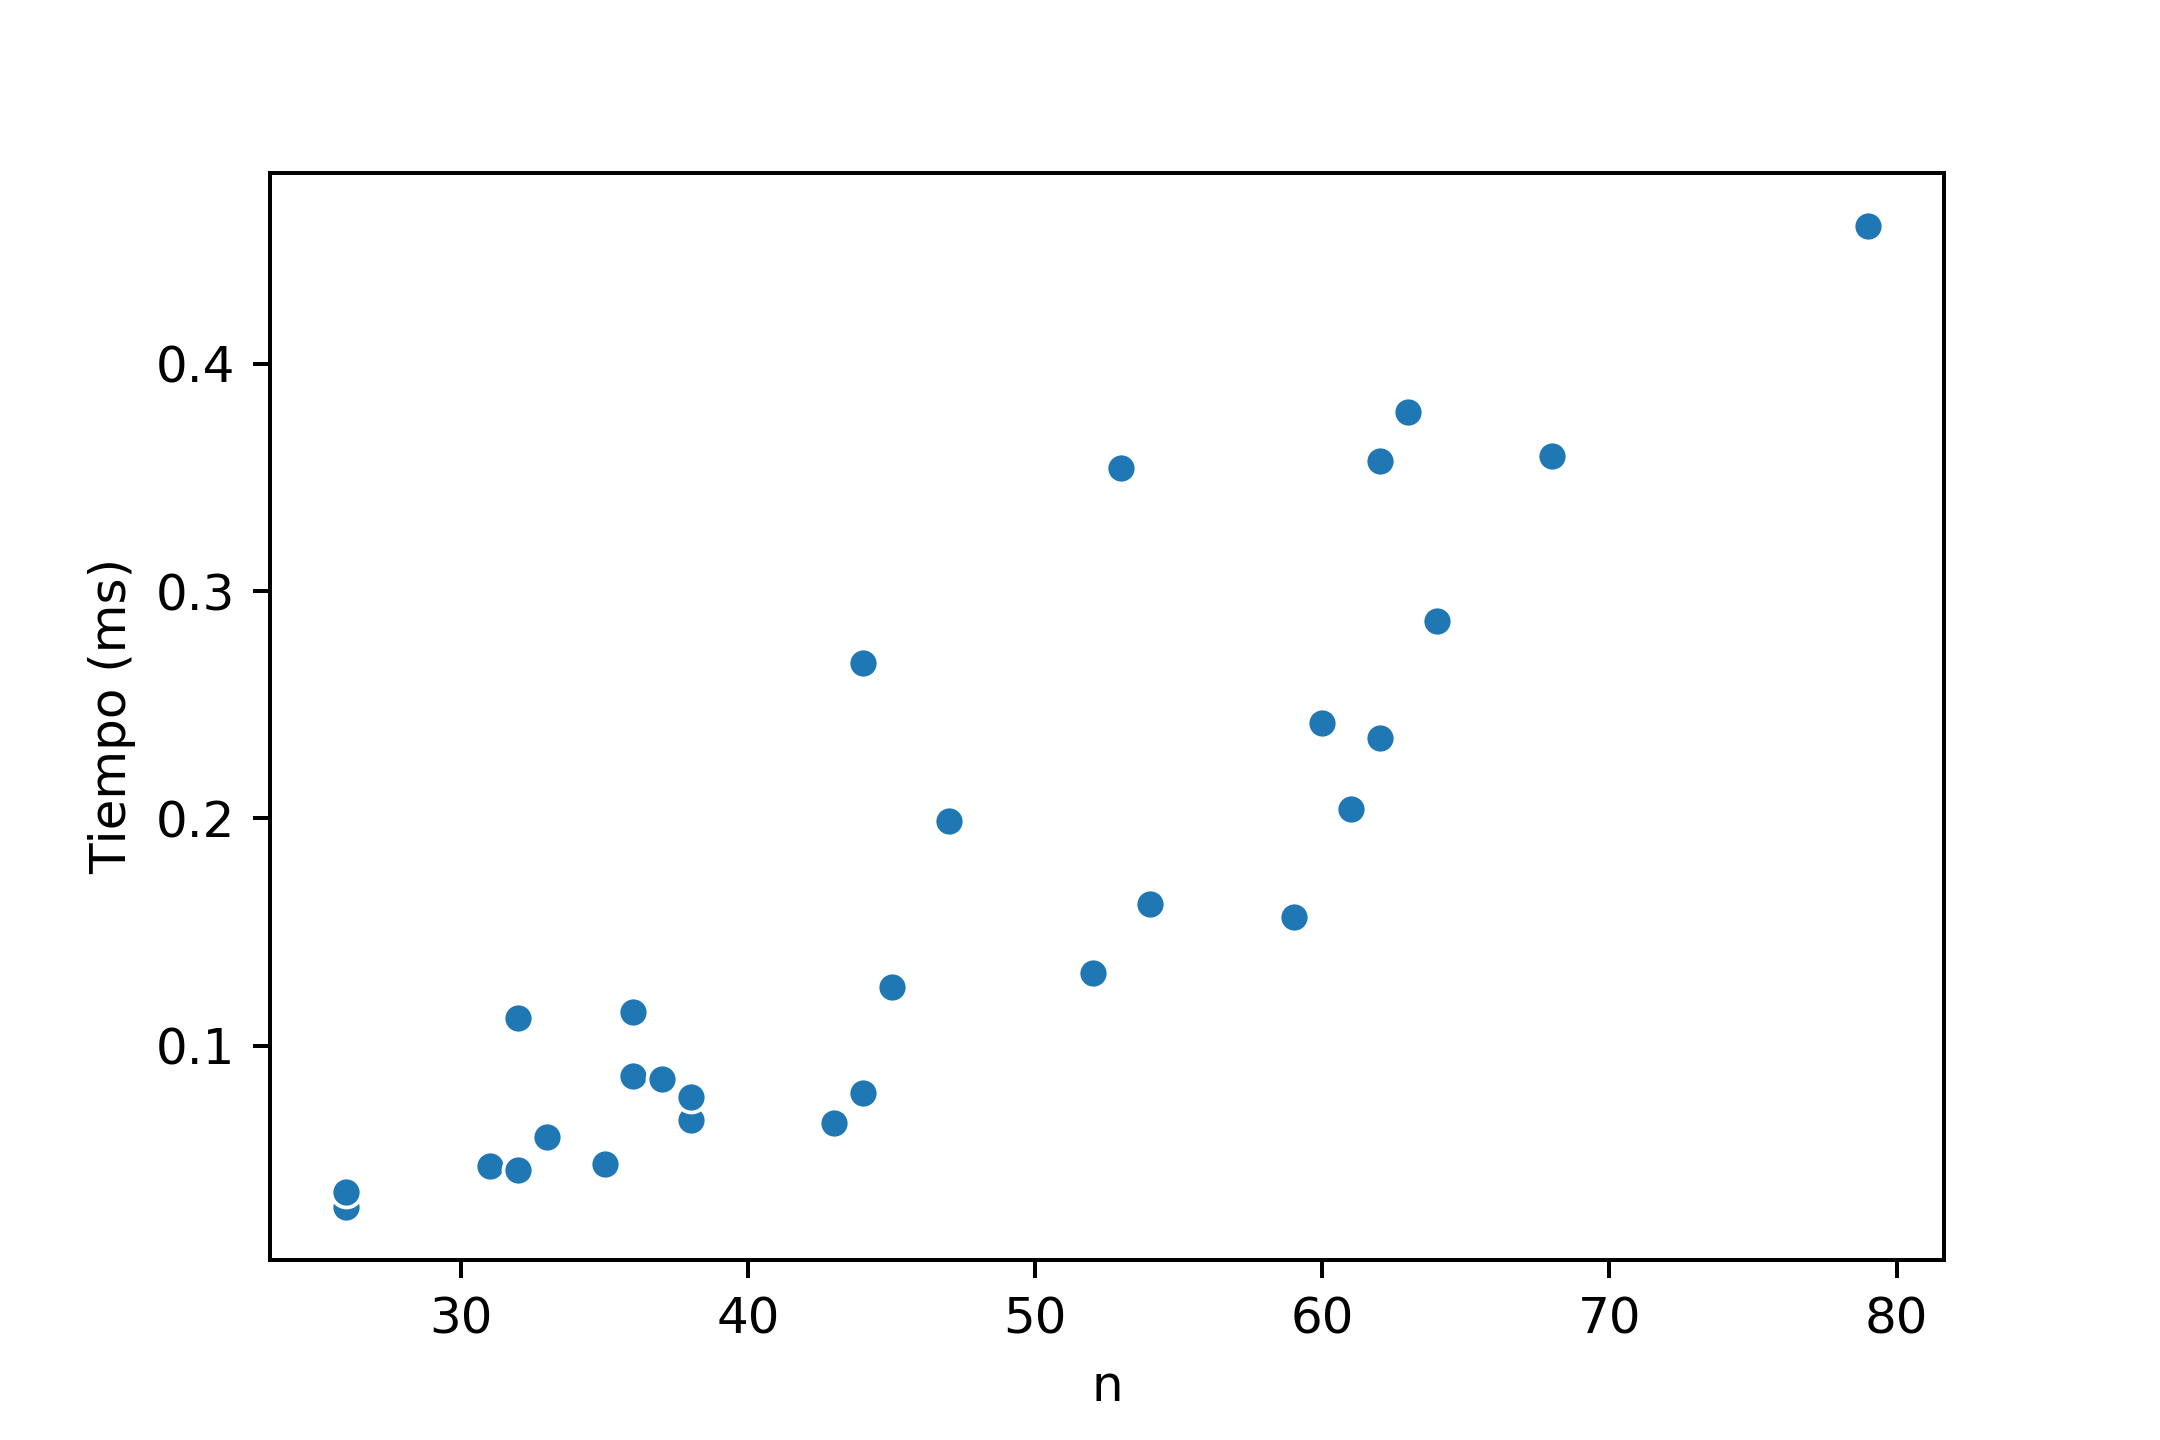
\includegraphics[width=1\textwidth]{images/kmeans/tiempokmeans}
		\caption{\footnotesize Tiempo de acuerdo al tamaño de la entrada}
		\label{fig:kmeans-tiempos}
	\end{minipage}%
	\hspace{0.03\textwidth}
	\begin{minipage}{0.45\textwidth}
		\centering
		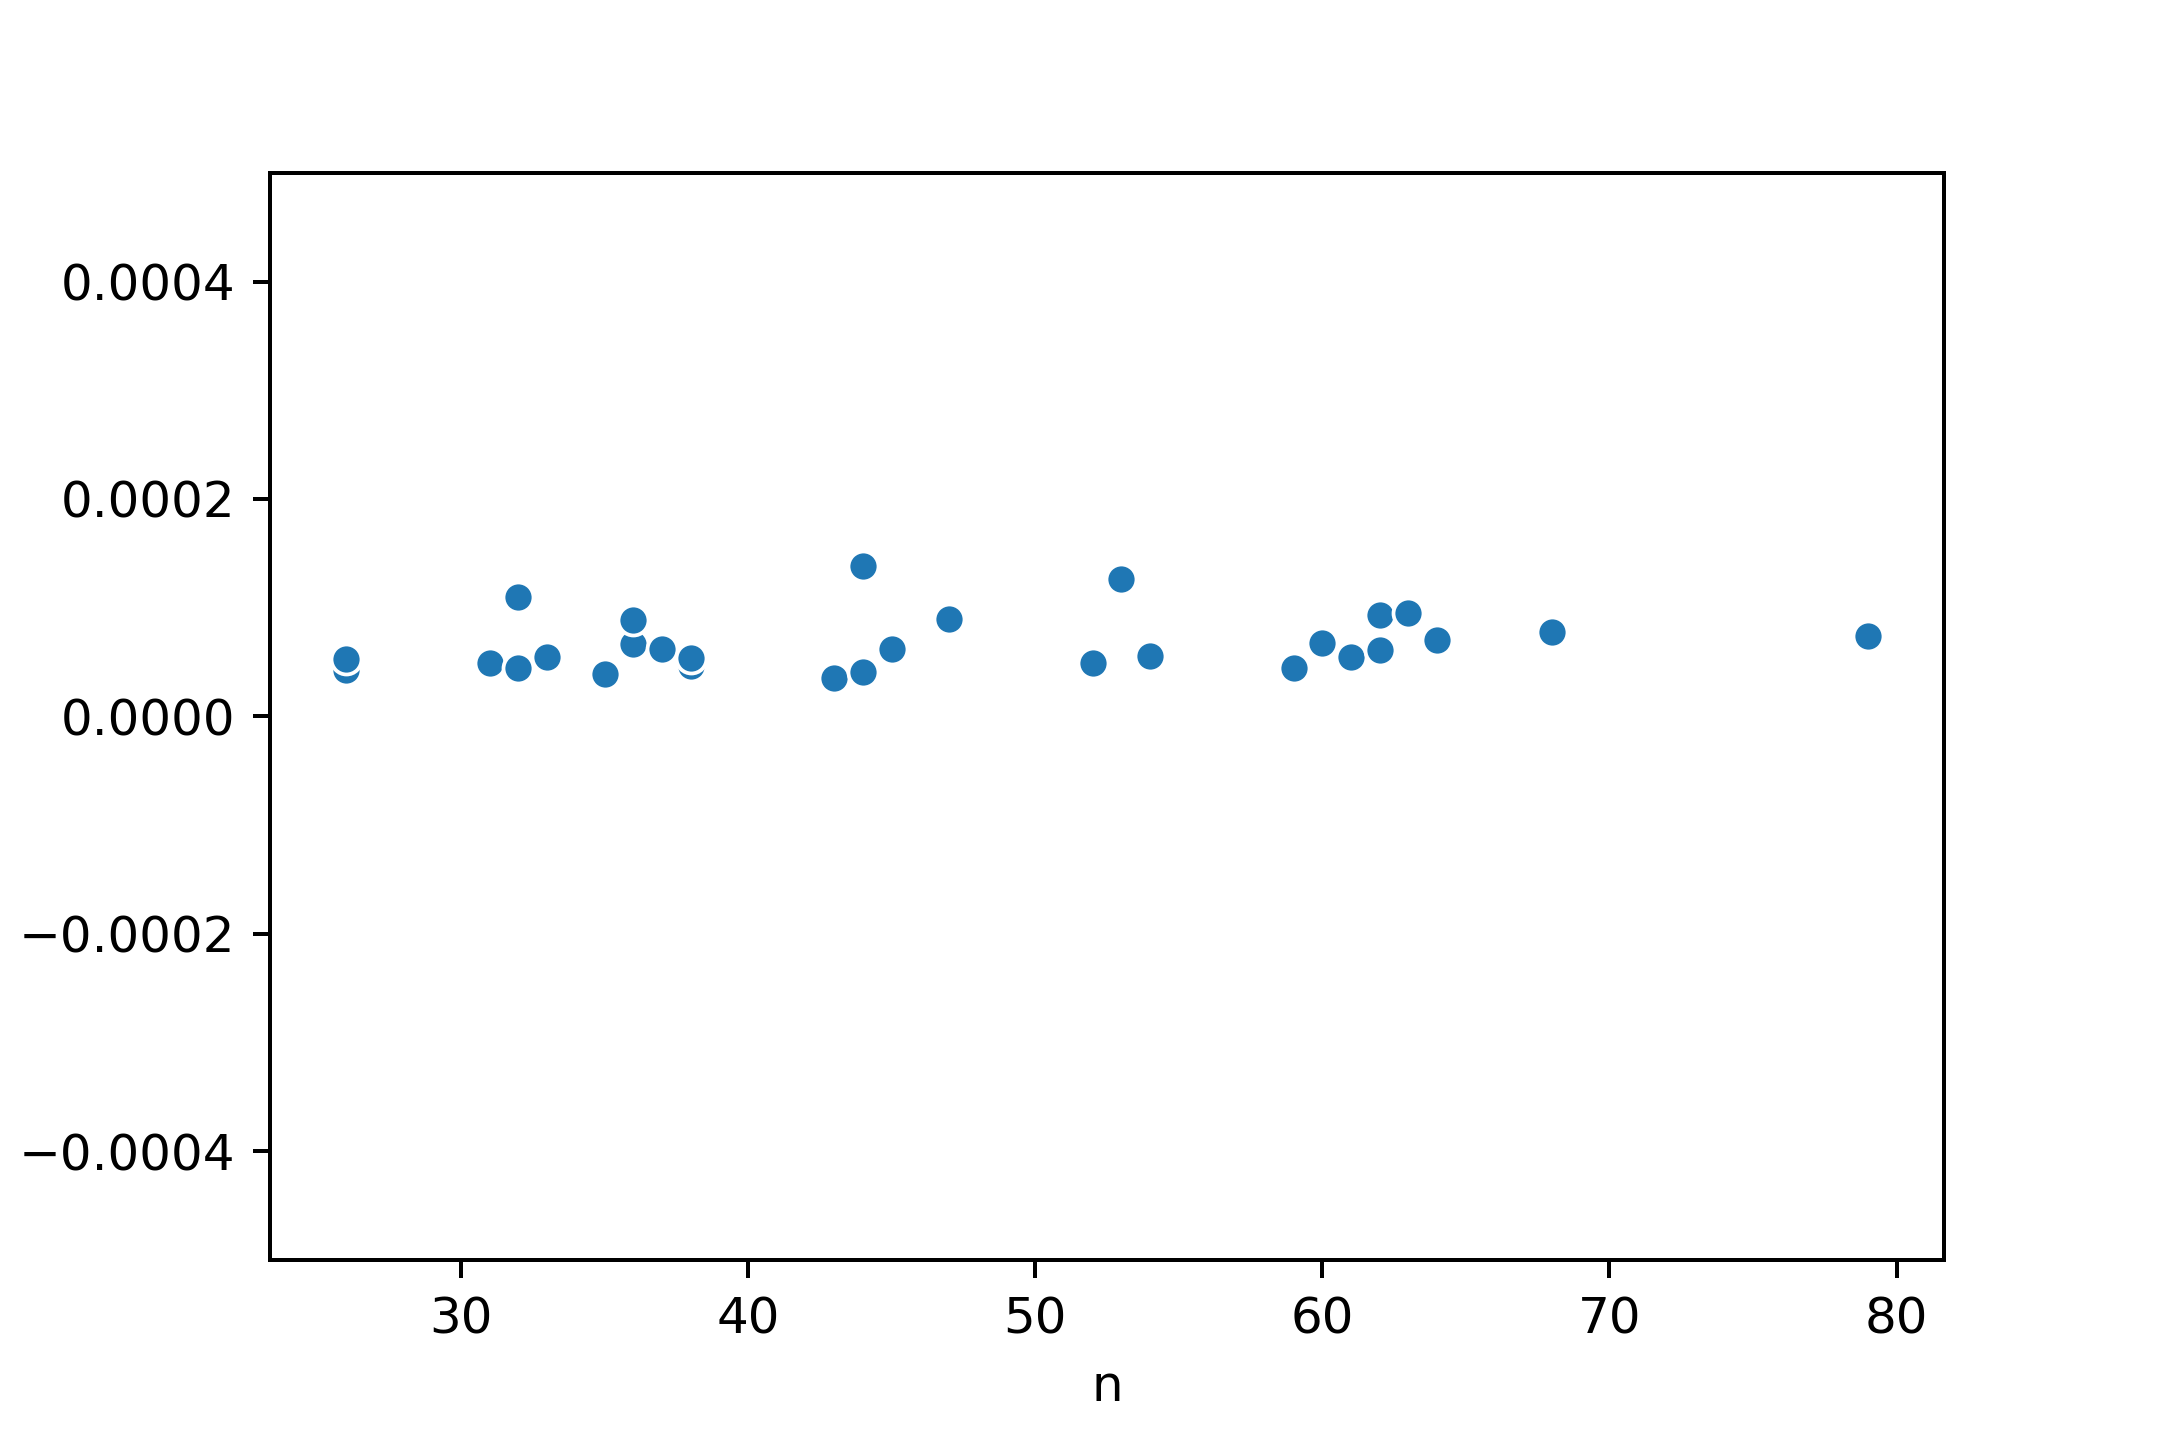
\includegraphics[width=1\textwidth]{images/kmeans/kmeanscte}
		\caption{\footnotesize Tiempo/complejidad de acuerdo al tamaño de la entrada}
		\label{fig:kmeans-cte}
	\end{minipage}%
\end{figure}

\paragraph{} 
En la figura \ref{fig:kmeans-tiempos} podemos ver como se comporta kmeans a medida que aumenta la cantidad de clientes. Como era de esperarse, se observa que no depende sólamente de $n$, hay una gran varianza entre los puntos más allá del tamaño de la entrada. Como dijimos, depende de la disposición de los puntos, de como esten distribuidas las demandas y de como se recorran los clientes. Por último en \ref{fig:kmeans-cte} se observa la relación entre la complejidad del algoritmo que habíamos calculado y el tiempo efectivo de las soluciones. Como es una recta que se mantiene constante, la complejidad puede ser acertada.



